%!TEX root = ../Master.tex
\chapter{Theory}

This chapter describes all theory needed in order to implement the solution presented in \cref{cha:solution} and why this theory is chosen. The chosen theory includes graph theory for modelling building complexes, wayfinding algorithms for searching through graphs find the most optimal route and how the general software architecture of the solution is.



% positioning is outcommented because it is not relevant theory for our solution
%%!TEX root = ../../Master.tex
\section{Triangulation}

\subsection{subsection name}

  \begin{figure}[ht!]
  \centering
  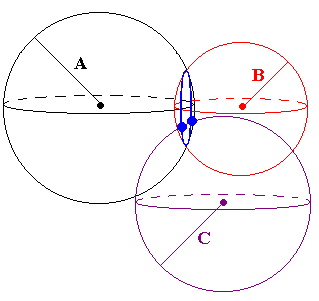
\includegraphics[width=3in]{trilateration}
  \caption{Example of lateration with three know positions.}
  \label{fig:trilateration}
  \end{figure}
  

  Trilateration in three dimensions is possible in fare most situations if and only if the distance to three known positions is defined or possible to calculate.
  If we know a distance to one of these three positions we know that the point we are seeking is in the surface of a sphere, with center at the know position, and with a radius equals to the distance to the center. This is illustrated on \cref{fig:trilateration} as the surface of the sphere A.

  The intersection of two spheres is a circle. By determining the distance to a second know point it is possible to circumscribe the range of possible position to a smaller area.
  This is illustrated as the blue circle on \cref{fig:trilateration}, and is the intersection between sphere A and B.
  A third sphere that overlaps the intersection between the first two spheres, will mark 2 points where all three spheres is collapsing. In fare most situations there are only one of these locations that lies on the Earth's surface, the other point will often be fare in to the sky or deep inside earth. So by sorting one point from, there is only one possible position left. 
  In some very rare situation it is possible that both point lies on the Earth's surface, and in such situations the use of four spheres will determine witch of the to positions is the right one.



\subsection{Angulation}


	\sinote{Needs introduction}

  For example, rangers in location known fire lookout towers can use AOA to pinpoint where the fire is. See \cref{fig:aoa} A ranger at tower A sees the fire and notates the bearing to the fire. He then communicates with a ranger at tower B telling him the general direction of the fire. The ranger at tower B now notates the bearing to the fire from his perspective. The fire can now be pinpointed from the 2 remote points (given the fire started in a 2-D world). The fire is where the 2 angle direction lines intercept A ranger at tower C can verify this position by also noting his bearing. \cite{compassdude_triangulation}

  \begin{figure}
    \centering
    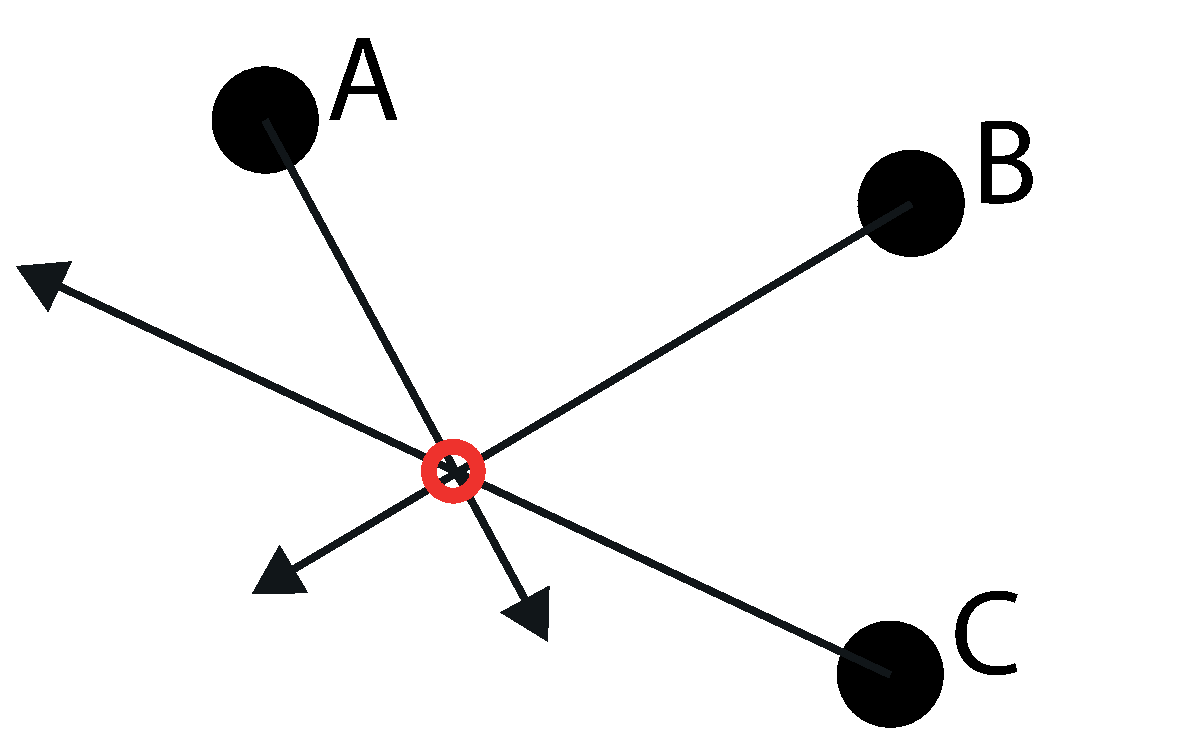
\includegraphics[width=\textwidth]{aoa.eps}
    \caption{Example of fire lookout towers positioning a fire using AOA.}
      \label{fig:aoa}
  \end{figure}

  The advantages of AOA are the few remote points needed in order to estimate a position. Another advantage is the independency of time synchronization.

  The disadvantages of AOA are the need of large and complex hardware requirements, and degradation of the location estimate as the target moves away from the measuring units. In order to perform accurate position of the target, very accurate angle measurements need to be performed. This can become a problem if the measuring is done in wireless networks, because of shadowing, multipath reflections arriving from misleading directions etc. Therefore angulation is best performed in free space.
%!TEX root = ../../Master.tex
\section{Graph theory}

Graph theory is frequently used in computer science to model some kind of relationship between objects. These objects could be anything. Graph theory is a preferred method to model building complexes, because it can precisely model how e.g. a hallway in a hospital is connected to a room.

In graph theory objects are called \enquote{nodes} or \enquote{vertices}. The two terms can be used interchangeably. In this paper, vertices will describe coordinates or POI (points of interest) in a hospital. Another term in graph theory is an edge. This is basically connecting two vertices and thereby providing a relationship between these vertices. See \cref{fig:labeled_graph}. An edge can be seen as a possible route connecting one coordinate to another. Now in order to describe the relationship between two vertices, we use an weighted graph in which an edge has a number attribute called a weight. A weight can describe the time, distance or any other metric that in some way can describe how two connected vertices are related.\cite{wiki_graph_glos,MIT2012}

We can describe these definitions formally.\cite{MIT2012}
\begin{mydef}
	A graph $G$ is a pair of sets $(V,E)$ where $V$ is a non-empty set of items called vertices or nodes. $E$ is a set of 2-item subsets of $V$ called edges.
\end{mydef}

\begin{figure}[ht!]
    \centering
    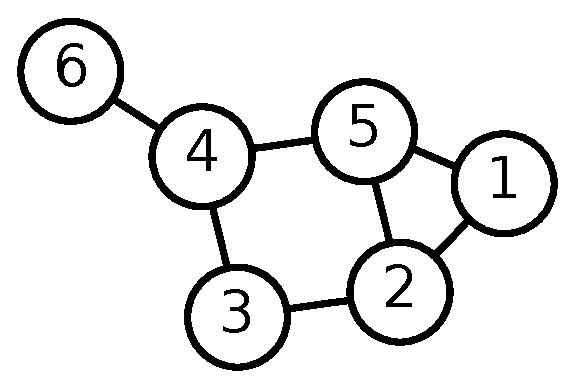
\includegraphics[width=0.5\textwidth]{6n-graf.eps}
    \caption{A labeled simple graph with vertex set $V = \left\{ {1, 2, 3, 4, 5, 6} \right\} $ and edge set $E = \left\{ \left\{ {1,2}\right\}, \left\{ {1,5}\right\}, \left\{ {2,3}\right\}, \left\{ {2,5}\right\}, \left\{ {3,4}\right\}, \left\{ {4,5} \right\} , \left\{ {4,6} \right\} \right\}$. \cite{wiki_graph_glos}}
    \label{fig:labeled_graph}
  \end{figure}

\subsection{Storing a complex as a graph}

\subsubsection{Representing a floor}

Every decision and every change direct is a vertex in our graph, is modelled by vertices connected with edges. Exits, elevators, stair and bridges are vertices for getting from a floor to another, including another building. Vertices that does not classify as one of the previously mentioned are doors, intersection and a change of walking direction. See \cref{fig:Vertices}. Connecting the vertices are edges with a weight, which could be weighted with the distance in meters from one vertex to another.

\begin{figure}[ht!]
    \centering
    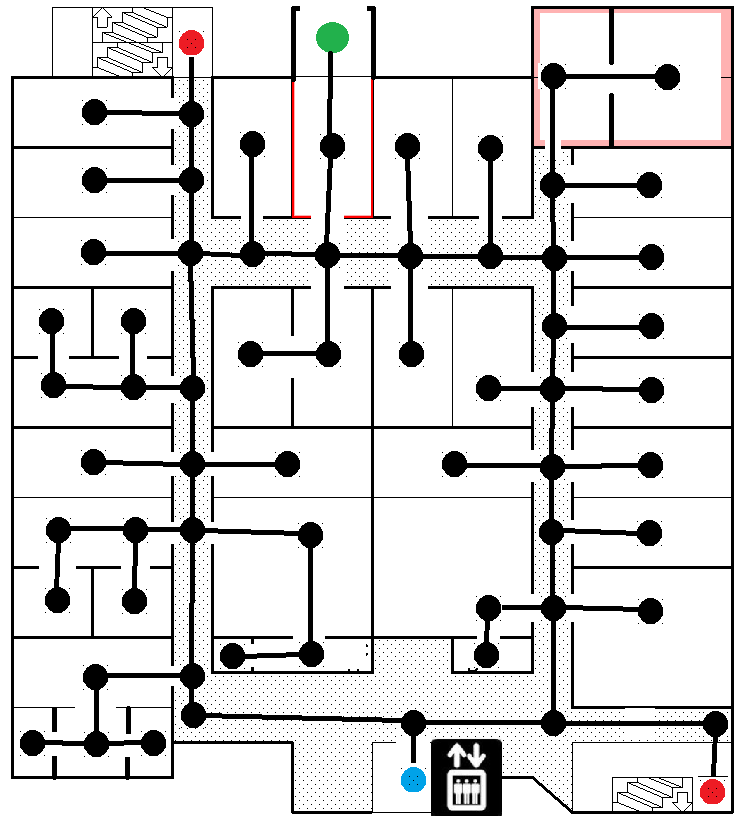
\includegraphics[width=0.5\textwidth]{floorplan_graf}
    \caption{Representation of a floor with graph}
    \label{fig:floorplan_graf}
  \end{figure}
\

\subsubsection{Multiple floors}

A complex such as a hospital usually consist of multiple floors, connected by stairs and elevators as observed at the visit to Sygehus Nord. Representing floors in a graph could be constructed by having edges in between floors. Elevators or stairs are represented by vertices that connects the edges between the floors. Having a graph that models the whole complex can have complications such as overlapping vertices coordinates. Estimating a heuristic value between destination and vertices on two separate floors, means that the heuristic models that does not account for obstacles, would cause the A* algorithm to expand vertices, leading to vertices below the destination on a separate floor than the desired. See \cref{fig:buildingAstar}.

\begin{figure}[ht!]
    \centering
    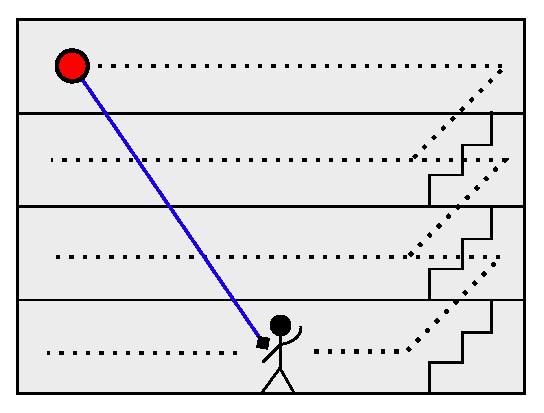
\includegraphics[width=0.5\textwidth]{buildingAstar}
    \caption{How many vertices the A* algorithm would expand, if using the euclidean distance as heuristic}
    \label{fig:buildingAstar}
  \end{figure}

If the complex is divided into separate floor graphs, the algorithm would not have to account for the height coordinates in its heuristic value. A algorithm could evaluate if the source and destination is on the same floor, if not the algorithm could divide the problem into A* searches. First finding a path leading to an elevator or stair which lead the destinations floor. The optimal path from one floor to another can be pre-calculated and stored. 

\subsubsection{Multiple buildings}

The previously described method for modelling floors allows the algorithm to comprehend from complexes of multiple buildings, as seen in \cref{fig:PekhoeS}. The numbers indicate the different floor id's and the letters indicates the connections between the floors. Connection d shows a curved line between 5 and 4 which means they are connected. Every vertex that connects a floor exit with another floor exit, is called a vertex exit\label{e_vertex}. \newline

If we have a building with three floors and one with two floors, the floors will be numbered 1,2,3,4 and 5. The building with the three floors would have its first floor numbered 1, second numbered 2 and last numbered 3. The building with two floors would have its first floor numbered 4 and second floor numbered 5. When modelled, the floors will sorted by their id (number) and stacked as seen on the figure. This means the second floor on two separate buildings will not have the same id. This simplifies a lookup if an individual is on the destination floor height physically, but not in the right building, because a the actual floor height is not relevant as they have been numbered. The thick straight line between 3 and 4, indicates a separation between two buildings. As seen on the figure, there is a exit vertex(a) at floor 1 making a connecting to 2, this could be because of a stair or elevator. The connection(c) between 1 and 4 is possible as both of these floors is at ground level. There is also a connection(b) between 2 and 5 even though the floors is not at ground level or in the same building, this could be they had a bridge leading between them, resulting in a connection. This allows for an exit from one building to another even though the user is not on the first floor. 
\annote{fig 4.4 boer vaere under Multiple buildings og ikke under Pathfinding Algorithms}
\begin{figure}[ht!]
    \centering
    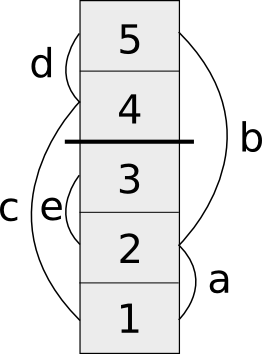
\includegraphics[width=0.5\textwidth]{PekhoeS}
    \caption{Visual representation of floors}
    \label{fig:PekhoeS}
  \end{figure}

%%!TEX root = ../../Master.tex

\section{Location Fingerprint}

  \subsection{K Nearest Neighbour}

  The k-nearest-neighbour (k-NN) algorithm simply compares a data set to $k$ closest-neighbour data sets, meaning data sets that are close to the original data set. The closeness is called the distance and is typically computed using the Euclidean distance or the Hamming distance.\cite{Liu2007, wiki_knn}

  In location fingerprinting, k-NN uses the online Received Signal Strengths (RSS) to find the closest $k$ locations from the a priori RSS.

%%!TEX root = ../../Master.tex
\subsection{Path finding Algorithms}

  Path finding algorithms are used for finding a path between two locations, the source and the destination. By searching its way from the source to the destination, until a path is found. These algorithms also make it possible to calculate the optimal path, i.e. the shortest.

  The algorithms to perform searches make use of a weighted graph. A graph, $G$ is a set of nodes $V$, connected by links $E$.
  Information about destinations, rooms, entrances and exits would be represented as nodes and hallways and stairs would be represented as links. The distance to travel from node to node via a particular link, would be represented as a weight $W(e)$.

  \begin{figure}[ht!]
    \centering
    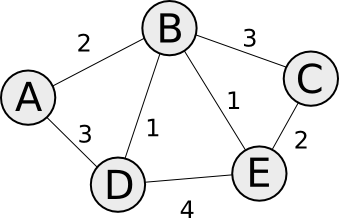
\includegraphics[width=\textwidth]{Graph}
    \caption{A Graph}
    \label{overflow}
  \end{figure}

  An important factor of a searching algorithm is correctness and also the time required to calculate the optimized path.
  The algorithms can be rated by their worst-case time, to ensure a responsive performance.

  \subsubsection{Dijkstra's Algorithm}

  A commonly used algorithm for finding the shortest path is Dijkstra's algorithm. It loops through steps until all nodes to the target node is optimized with the least cost, then points out the shortest path from source node, to target node. Because of the need of every node being evaluated, the complexity of algorithm is proportional to the number of nodes, which means that a lot of computational power is required to calculate the result. \sinote{Vis kompleksitet med store O notation?} \cite{Dijkstra}

  \begin{figure}[ht!]
    \centering
    \frame{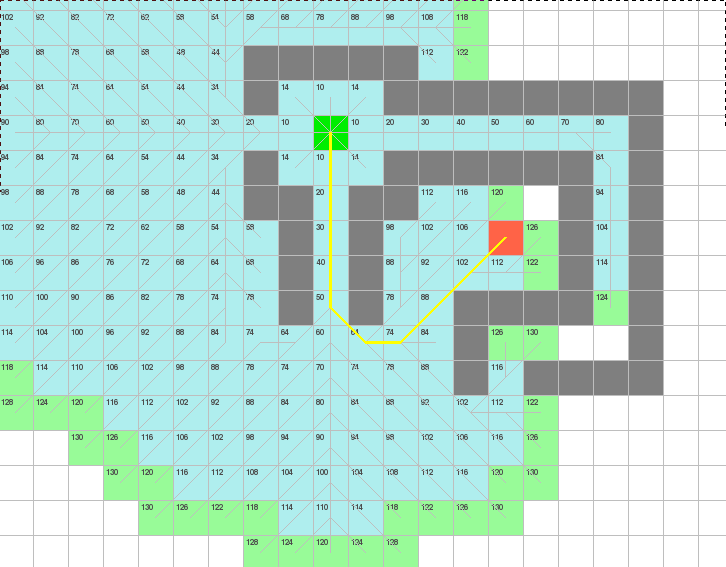
\includegraphics[width=\textwidth]{Dijkstra}}
    \caption{Dijkstra's algorithm in action}
    \label{overflow}
  \end{figure}

  We consider the problem: find shortest path from source to target.

  Where $P$ is the source node, $Q$ is the target and $R$ is the evaluating node.

  The nodes are subdivided into three sets:

\sinote{Forslår description environment her. Skaber mere overblik}
  Set $A$ - Optimized nodes (least costly path from $P$ is known)
  Set $B$ - Temporary nodes (evaluated cost of path from $P$ but not part of set $A$)
  Set $C$ - Remaining nodes

  The links are subdivided into three other sets:

\sinote{Forslår description environment her. Skaber mere overblik}
  Set \RN{1} - Links used in the set $A$
  Set \RN{2} - Not part of set I (one and only one link of this set will lead to each node in set $B$)
  Set \RN{3} - Remaining links (rejected or not yet considered)

  At first all nodes is assigned to set $C$ and all links to set \RN{3}, P is then assigned to set $A$.
  Then we loop through following steps until $Q$ is part of set $A$.

\sinote{Forslår description environment her. Skaber mere overblik}
  Step 1. Consider all the links r connecting the node just assigned to set $A$. If $R$ is part of set $C$ assign to set $B$ and assign r to set \RN{2}. \sinote{simon: R eller r?}
  If R is part of set $B$, then investigate if the use of link r is less costly from $P$ to R than the existing link in set \RN{2}. If less costly assign link r and reject existing link in set \RN{2}, otherwise reject r to set \RN{3}.

  Step 2. For each node in set $B$ where there is only one path in set \RN{1} and set \RN{2}, the node with minimum cost from $P$ is assign to set $A$ and with the corresponding link assign to set \RN{1}.

  \begin{figure}[ht!]
    \centering
    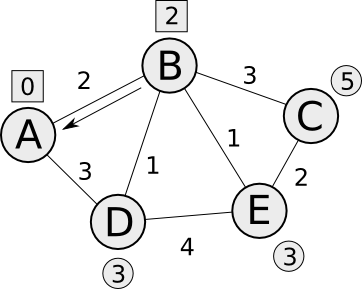
\includegraphics[width=\textwidth/3]{DijkstraX}
    \caption{Dijkstra calculation}
    \label{overflow}
  \end{figure}

  \subsubsection{Best-First-Search}

  Best-First-Search is search algorithm like Dijkstra's algorithm, with the exception that is uses heuristic to estimate how far target the node is the an evaluating node, then it repeatedly choose the node with the least cost, until target node is reached. \sinote{nok bedst du selv lige læser denne sætning igennem igen. Skal måske omformuleres} The final path is not guaranteed the shortest, however it it not as complex as Dijkstra's algorithm which means it is much faster to calculate. \cite{BestFirst}

  But when obstacles are introduced, like walls, the Best-First-Search algorithm fails to find a path that is close to optimal.

  \begin{figure}[ht!]
    \centering
    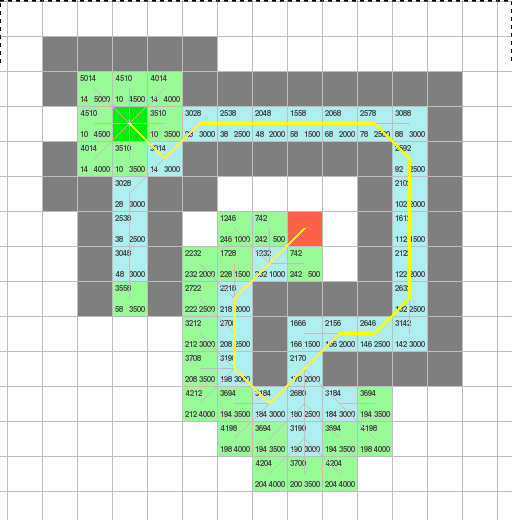
\includegraphics[width=\textwidth]{BestFirst} 
    \caption{Best-First-Search in action}
    \label{bestfirst}
  \end{figure}

  \subsubsection{A* Algorithm}

  If you would combine Dijkstra's algorithm with Best-First-Search algorithm, you would get the A* algorithm which also utilises the principle of a heuristic estimation to determine which node to test next. It uses a evaluation function $f(x) = g(x) + h(x)$, where $g(x)$ describes the cost from the start to the node being evaluated, and $h(x)$ is a heuristic function that estimates the cost from the evaluating node to the target node. \cite{http://theory.stanford.edu/}

\sinote{brug evt itemize}
  - If $h(x)$ is zero, then only $g$ affects the result and making it work like Dijkstra's algorithm.

  - If $h(x) < g(x)$, the algorithm will guaranteed find the shortest path from source to target, at a slow running time.

  - If $h(x) == g(x)$ \sinote{bare = i stedet for ==?}, the algorithm will only extract the best path, but this not always possible due to obstacles.

  - If $h(x) > g(x)$, the algorithm will find a path fast not its not always the optimal, then works like the Best-First-Search algorithm.\sinote{skal måske omformuleres?}

  This means that the heuristic estimation should be reasonable, $h(x)$ should be admissible and not overestimate the distance between the evaluating node and the target node. But should be just right for the final chosen path to be the optimal path and the for the complexity of the algorithm to be at a minimum. Each step the algorithm evaluates the value of $f(x)$ of each node to pick the next node with the smallest cost.

  \begin{figure}[ht!]
    \centering
    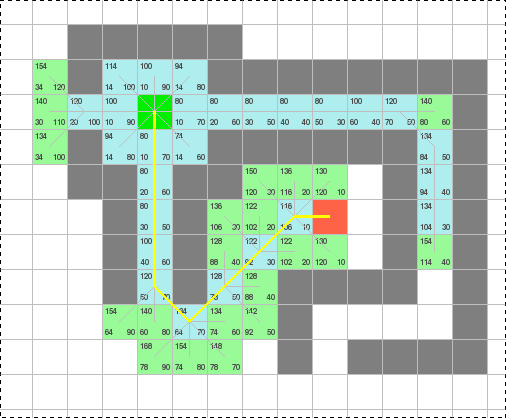
\includegraphics[width=\textwidth]{AstarHlow}
    \caption{A* algorithm with an admissible heuristic value}
    \label{astar}
  \end{figure}

  There is multiple ways to calculate the heuristic value(estimated cost) to the target node, but an ideal choice would be the Euclidean \ref{equation:Euclidean} \sinote{brug evt. cref i stedet. Den indsætter selv eq. og nummer.} distance, as no path can be shorter than the direct distance between two nodes.
  \begin{equation} \label{equation:Euclidean}
    dist((x, y), (a, b)) = \sqrt{(x - a)^2 + (y - b)^2}
  \end{equation}

  \subsubsection{Summary of Algorithms}

  Path algorithms searches for a path to target. Some focuses on finding a path fast, others finding the most optimal path. Using the A* algorithm with a heuristic model that is admissible, which underestimates the cost to the target path, assure an optimal path without calculating every node. See \cref{tbl:scheme}
  
  \begin{table}[ht!]
    \centering
  \rowcolors{1}{}{lightgray}
    \begin{tabular}{|r|l|c|}
      \hline
      \textbf{Algorithm} & \textbf{Advantages} & \textbf{Disadvantages} \\
      \hline
      Dijkstra's & Always optimal path & Slow calculation \\
      Best-First-Search & Fast calculation & Not always optimal path \\
      A* & Optimal path if $h(x)<g(x)$, Fast calculation & Not always optimal path \\
      \hline
    \end{tabular}
    \caption{Table of advantages/disadvantages of different algorithms}
    \label{tbl:scheme}
  \end{table}
%!TEX root = ../../Master.tex
\section{Algorithms for pathfinding}
Graph Search Algorithms analyses the structure of a graph. This can be used to find the shortest path from one vertex to another, in a graph \cite{Cormen2009}. Some graph search algorithms are more efficient than others, at finding the shortest path connecting two vertices in a graph.

Finding the shortest path from one vertex to another, is defined as a single-pair shortest path (SPSP) problem. Finding the shortest path from a single source vertex to all other vertices, is defined as a Single Source Shortest Path (SSSP) problem.


This section describes both Dijkstra's algorithm , which is used for solving SSSP problems, in \cref{subs_dijkstra}, and the A* algorithm, which is used for solving SPSP problems, in \cref{subs_astar}. These algorithms are very alike, but they each differ in a few important ways. They will both always find the shortest path, however Dijkstra's is inefficient in terms of speed, while the A* algorithm is dependent on an admissible heuristic. This is explained in \cref{subs_astar}.

%   In \cref{sec:specification} we specified that our solution needs to find the shortest weighted path to the destination.
%   To better understanding pathfinding we examined different algorithms. We discovered that some algorithms have a high accuracy but is slow at finding the path, and conversely.
%   We have compared some well known path finding algorithms by evaluating their calculation time and route precision.

%   In the following we compare 3 frequently used algorithms:
%   \begin{itemize}
%     \setlength{\itemsep}{1pt}
%     \setlength{\parskip}{0pt}
%     \setlength{\parsep}{0pt}
%     \item \textbf{Dijkstra's Algorithm} Always finds the shortest path but has long calculation time on more complex graphs.
%     \item \textbf{Greedy Best-First-Searches} Is a very fast algorithm but does not always find the shortest path.
%     \item \textbf{A* Algorithm} Is an extension of Dijkstra's Algorithm but has less calculation time using heuristic values.
% \end{itemize}

% The A* algorithm was chosen as the algoritm of choice because it always finds the shortest path, and still has a reasonable fast computing time. This algorithm also makes it easier to implement stairs and elevators, because of the heuristic values. In this section we will describe A* and Dijkstra's because A* is an extension of Dijkstra's.


  %Path finding algorithms are used for finding a path between two locations, the source and the destination. By searching its way from the source to the destination, until a path is found. These algorithms also make it possible to calculate the optimal path, i.e. the shortest. \cite{Cormen2009}


  % \begin{figure}[ht!]
  %   \centering
  %   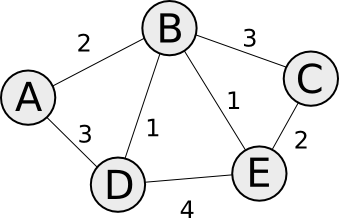
\includegraphics[width=0.5\textwidth]{Graph}
  %   \caption{Weighted graph}
  %   \label{fig:graph}
  % \end{figure}

  %An important factor of a searching algorithm is correctness and also the time required to calculate the optimized path. The algorithms can be rated by their worst-case time, to ensure a responsive performance.

  \subsection{Dijkstra's Algorithm}\label{subs_dijkstra}

  Because every vertex needs to be evaluated the complexity of Dijkstra's algorithm is proportional to the number of vertices.This means that a lot of computational power is required to calculate the result \cite{Dijkstr1959}.

  An example of Dijkstra's algorithm in use is showed in \cref{fig:dijkstra}. Grey blocks are obstacles such as walls. White blocks are unvisited vertices. S marks the start and G the destination. Blue blocks mark vertices that were added to closed set (were visited) and green blocks mark vertices that were added to open set (were considered to be added to closed set). The A marks a point that illustrates that many unnecessary vertices are calculated using Dijkstra's algorithm. B marks a point that shows that Dijkstra's algorithm does consider in which direction the destination is. It keeps searching the graph uninformed until it has visited all vertices in the graph, that is was able to reach from the given source.


  \begin{figure}[ht!]
    \centering
    \frame{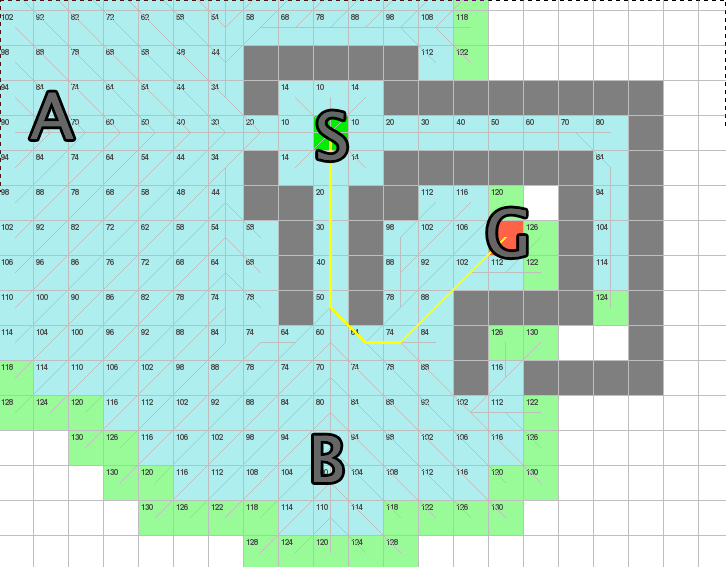
\includegraphics[width=0.5\textwidth]{Dijkstra_edited}}
    \caption{Dijkstra's algorithm in action}
    \label{fig:dijkstra}
  \end{figure}

\subsubsection{Pseudocode}

\Cref{algo:Dij} is a pseudocode example of Dijkstra's algorithm \cite{wiki_dijkstra}. 

\kanote{2: stack gør hvad?}

\begin{algorithm}
  \caption{Dijkstra's Algorithm}\label{algo:Dij}
  \KwResult{Finds the shortest path from start vertex to vertices}
  \KwData{\\
  graph \tcc*{graph being searched}
  source \tcc*{the source vertex}
  dist \tcc*{list of distances from source}
  visited \tcc*{list of visited vertices}
  parent \tcc*{list of parents. The parent of a given vertex, is another vertex that provides the shortest current path to the given vertex}
  E-list \tcc*{A list of vertices to be evaluated}
  E-vertex \tcc*{vertex being evaluated}
  C-vertex \tcc*{current vertex}
  Temp \tcc*{a temporary variable}
  }

  \SetKwFunction{Dijkstra}{Dijkstra}
  \SetKwProg{KwFn}{Function}{}{}

  \KwFn{\Dijkstra{graph, source}}{

    \For{\textbf{each} vertex v in graph}{
      dist[E-vertex] $= \infty$\tcc*{Assign distance from source to as infinite}
      visited[E-vertex] $=$ false\tcc*{Boolean to false for not visited}
      parent[E-vertex] $=$ undefined\tcc*{Assign parent all as undefined}
    }

    dist[$source$] $= 0$\tcc*{Source dist has distance 0}
    insert $source$ in E-list\tcc*{Source dist has distance 0}

    \While{E-list \textbf{is not} empty}{
      C-vertex $=$ E-vertex in E-list with lowest dist[]\tcc*{The new C-vertex is the vertex with lowest dist value}
      remove C-vertex from E-list\tcc*{Remove vertex C-vertex from E-list}
      visited[C-vertex] $=$ true\tcc*{Mark the new vertex C-vertex as visited}

      \For{\textbf{each} neighbour n of C-vertex}{
        $Temp =$ dist[C-vertex] + distBetween(n, C-vertex)\tcc*{Assign temp to the distance from $source$ to C-vertex plus the distance between n and C-vertex}
        \If{$Temp$ < dist[n]}{
          dist[n] $= Temp$\tcc*{Assign $Temp$ as the new shortest distance of vertex n}
          parent[n] $= u$\tcc*{Assign C-vertex as parent of vertex n}
          \If{n \textbf{is not} visited}{
            insert n into E-list\tcc*{Add the unvisited vertex n into the E-list to be evaluated}
          }
        }
      }
    }
    return dist\tcc*{Return the distances in dist}
  }
\end{algorithm}

When Dijkstra's algorithm has been performed, the optimal paths can be induced by backtracking. See \cref{algo:FindPath}.

\begin{algorithm}
  \caption{Find path to target}\label{algo:FindPath}
  \KwResult{Finds the shortest path from start vertex to a target vertex}
  \KwData{\\
        stack \tcc*{Sequence of vertices in path}
        target \tcc*{Evaluating vertex}
        source \tcc*{Source vertex}
        parent \tcc*{A list of parents}
   }

  \SetKwFunction{FindPath}{FindPath}
  \SetKwProg{KwFn}{Function}{}{}

  \KwFn{\FindPath{parent, source, target}}{
    $stack =$ empty sequence\;
    \While{parent[target] \textbf{is not} source}{
      insert $u$ in stack\tcc*{Insert u vertex in the stack}
      target $=$ parent[target]\tcc*{Traverse from target to source}
    }
    return $stack$
  }
\end{algorithm}

\subsubsection{An example of Dijkstra's algorithm in use}\label{subss_dij_ex}

The following steps explains how Dijkstra's algorithm is executed. The example graph is \cref{fig:graph}.

  \begin{figure}[ht!]
    \centering
    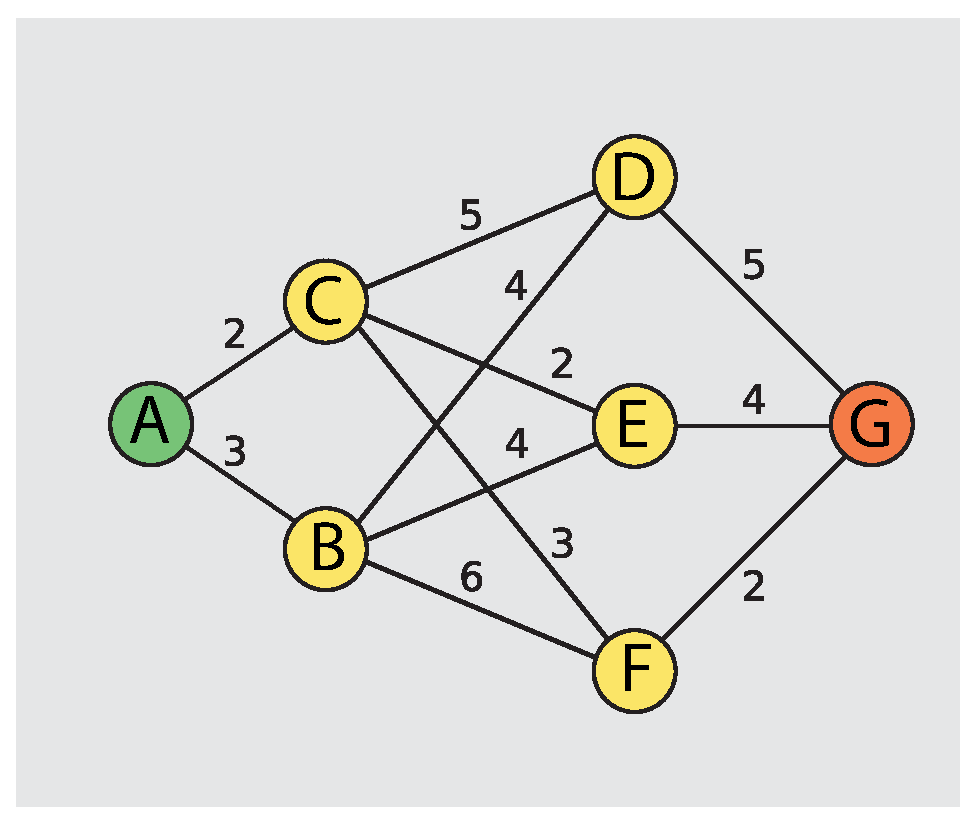
\includegraphics[width=0.5\textwidth]{eksempel_graf.eps}
    \caption{The example graph}
    \label{fig:dij_example_graph}
  \end{figure}

  \paragraph{Step 1}
Set the temporary distance of every vertex in the graph to infinity. The starting vertex should however be set to zero. See \cref{fig:dij_step1}.

  \begin{figure}[ht!]
    \centering
    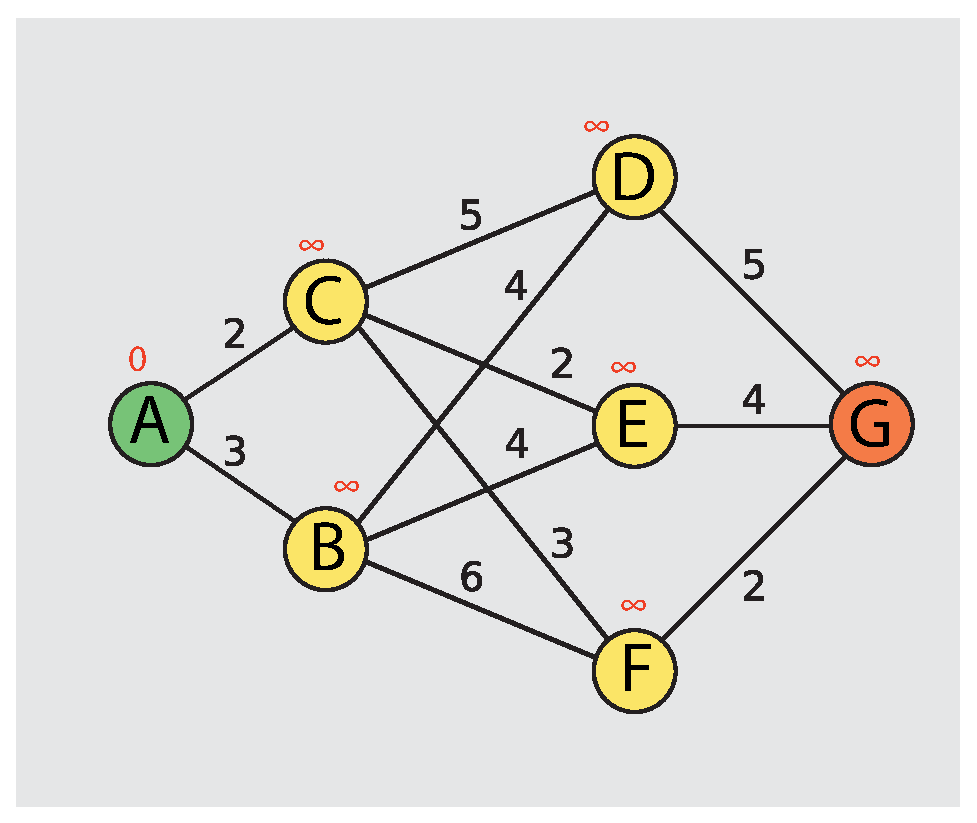
\includegraphics[width=0.5\textwidth]{dij_step1.eps}
    \caption{Step 1 of Dijkstra}
    \label{fig:dij_step1}
  \end{figure}

    \paragraph{Step 2}
Add every vertex to a set called unvisited vertices. Mark the starting vertex as current.

    \paragraph{Step 3}\label{par:dij_step3}
Calculate temporary distances for every neighbour of the current vertex. This is done by adding the distance of the current vertex and the weight of the edge connecting it to the neighbour. See \cref{fig:dij_step2-3}.

  \begin{figure}[ht!]
    \centering
    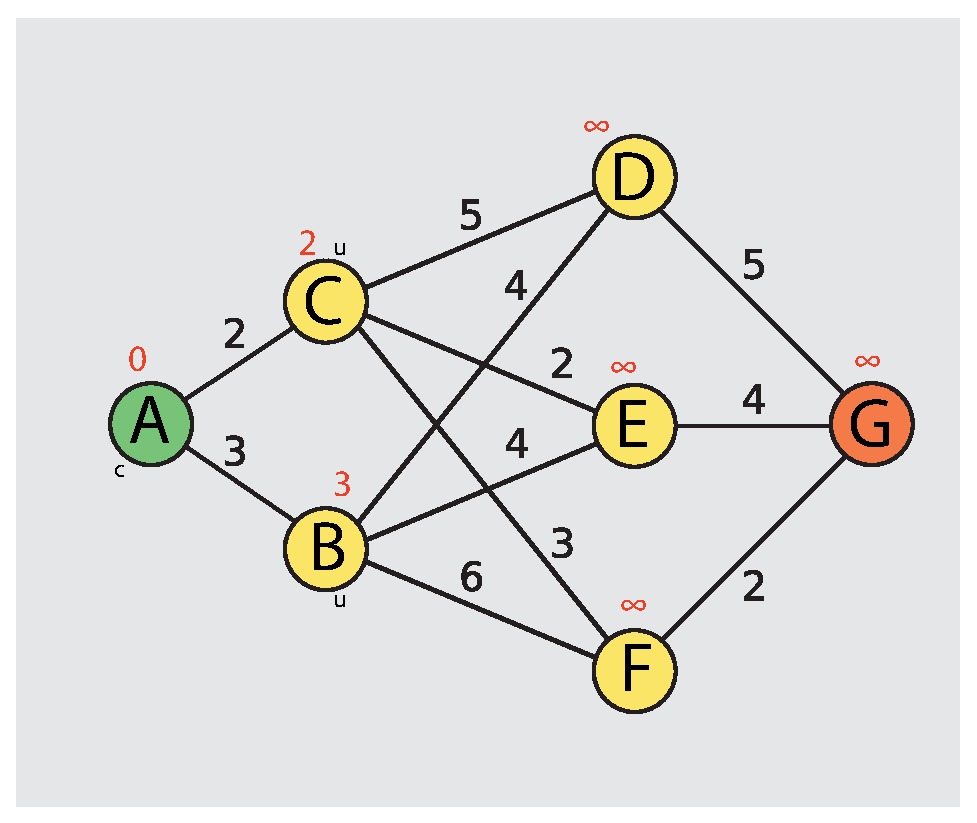
\includegraphics[width=0.5\textwidth]{dij_step2-3.eps}
    \caption{Step 2 \& 3 of Dijkstra. c marks the current vertex. u marks unvisited vertices.}
    \label{fig:dij_step2-3}
  \end{figure}

      \paragraph{Step 4}
When all neighbours have been considered, mark the current vertex as visited, thereby removing it from the set unvisited vertices. This visited vertex will then never be checked again. 

\paragraph{Step 5}
If all vertices have been marked visited or the smallest temporary distance in the unvisited vertices set is infinity, stop the algorithm. The smallest temporary distance in the unvisited vertices set should only be infinity if there is no connecting from starting vertex to destination vertex.

\paragraph{Step 6}
From the unvisited vertices set, select the vertex with the smallest temporary vertex as the current vertex. Repeat step 3 and onwards. See \cref{fig:dij_step4-5-6}.

  \begin{figure}[ht!]
    \centering
    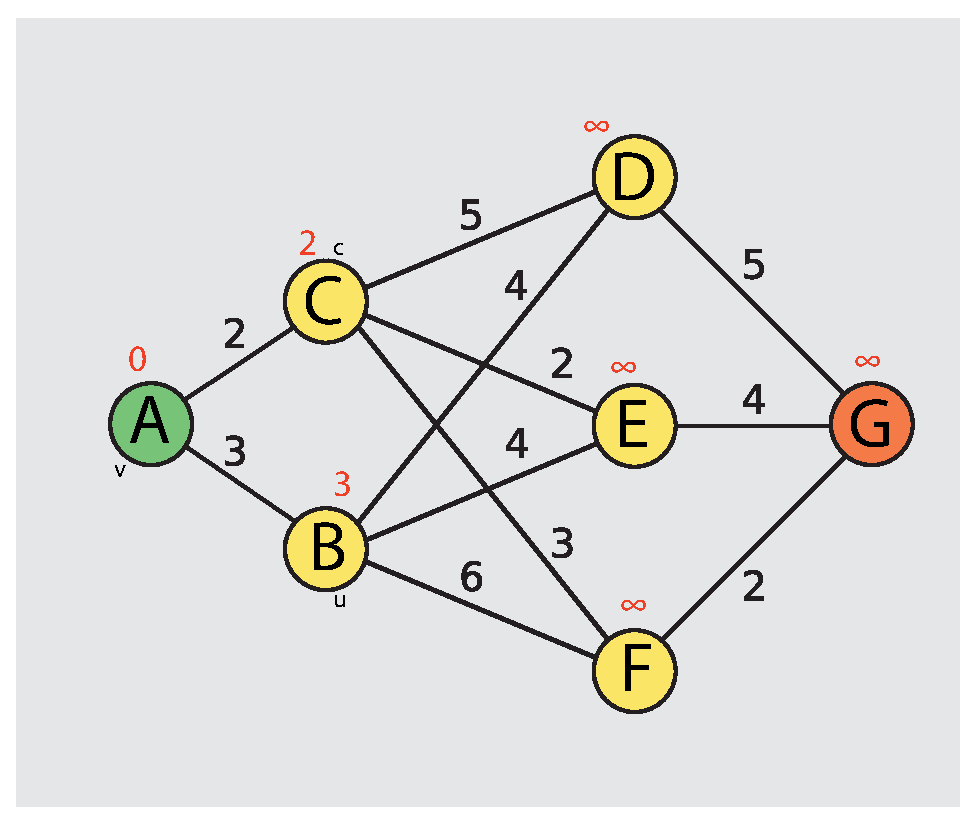
\includegraphics[width=0.5\textwidth]{dij_step4-5-6.eps}
    \caption{Step 4, 5 \& 6 of Dijkstra. c marks the current vertex. u marks unvisited vertices.}
    \label{fig:dij_step4-5-6}
  \end{figure}


  \subsection{A* Algorithm}\label{subs_astar}


  The A* algorithm is an extension of Dijkstra's algorithm providing better performance in terms of speed, while still maintaining the correctness of Dijkstra's algorithm, given an admissible heuristic value. An admissible heuristic value is explained below.

 
  \subsubsection{Heuristic value and evaluation value}
  A* introduces a heuristic value, which is an estimation of total cost from the source to the destination. For it to be admissible, the heuristic value must be exactly equal to or lower than the actual total cost from the source to the destination. If the heuristic value overestimates the cost, A* is not guaranteed to find the shortest path. The lower the heuristic value is compared to the cost value, the less influential the heuristic value is. If the heuristic value is completely without influence, A* performs like Dijkstra's algorithm.

  There are many different methods used to find a heuristic. Two commonly used methods are the Manhattan method and the Euclidean method. 

    \paragraph{Euclidean distance}\cite{wiki_euclidean}

  \[
    dist(p, q) = dist(q, p) = \sqrt{(q_{1} - p_{1})^2 + (q_{2} - p_{2})^2 + \dots + (q_{n} - p_{n})^2}
  \]

  Where $p$ and $q$ both are vertices in a graph. $p_{n}$ and $q_{n}$ are the coordinates of each vertices. For example $p_{1}$ is the $x$ coordinate of vertex $p$.

    \paragraph{Manhattan distance}\cite{wiki_manhattan_distance}

  \[
    dist(p, q) = dist(q, p) = \| \mathbf{p} - \mathbf{q} \| = \sum\limits_{i=1}^n | \mathbf{p_{i}} - \mathbf{q_{i}} |
  \]

  Where $p$ and $q$ both are vertices in a graph. $p_{n}$ and $q_{n}$ are the coordinates of each vertices. For example $p_{1}$ is the $x$ coordinate of vertex $p$.


  The heuristic value is used to determine the evaluation value. The evaluation value is found by adding the cost from the start vertex to the vertex being evaluated, to the heuristic value. The cost is the total sum of weights of edges visited to the vertex being evaluated. The evaluation value is used when determining if a vertex is in the shortest path. When comparing two vertices, the vertex with the lowest evaluation value is always chosen for the shortest path \cite{Patel2013}.


  For an example of an A* calculation, see \cref{fig:astar}. 
  Grey blocks are obstacles such as walls. White blocks are unvisited vertices. S marks the start and G the goal. Blue blocks mark vertices that were added to closed set (were visited) and green blocks mark vertices that were added to open set (were considered to be added to closed set). A marks a point where the heuristic value increases because the distance to G increases, causing the evaluation value to rise above the threshold for when A* considers another path. Point B marks a point where A* chooses a path around an obstacle.

    \begin{figure}[ht!]
    \centering
    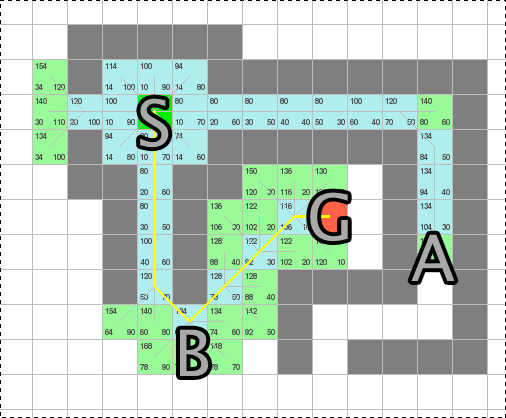
\includegraphics[width=0.5\textwidth]{AstarHlow_kopi.png}
    \caption{Example on an A* algorithm algorithm}
    \label{fig:astar}
  \end{figure}



  % If you would combine Dijkstra's algorithm with Best-First-Search algorithm, you would get the A* algorithm which also utilises the principle of a heuristic estimation to determine which vertex to test next. It uses a evaluation function $f(x) = g(x) + h(x)$, where $g(x)$ describes the cost from the start to the vertex being evaluated, and $h(x)$ is a heuristic function that estimates the cost from the evaluating vertex to the target vertex. \cite{Patel2013}

%\kanote{A WILD DESCRIPTION APPEARS! (referer!)}

\subsubsection{Pseudocode}

A* works by maintaining a priority queue of vertices that need to be examined. This is called the open set. The lower the evaluation value of a vertex is, the higher the priority in the open set. The current vertex is chosen as the vertex with the highest priority in the open set. This vertex is then removed from the open set and its neighbours' evaluation and closedSet values are updated. The neighbor's parent is marked as the current vertex. These neighbours are then added to the open set. The algorithm stops when either the open set is empty or the goal vertex has a lower evaluation value than any other vertex in the open set. If this happens the shortest path to the goal vertex has been found.

The shortest path is then backtracked by starting from the goal vertex and then traversing the goal's parent until the start vertex has been met. These vertices mark the shortest path.

\begin{algorithm} 
  \caption{A* Algorithm}\label{algo:A*}
  \KwResult{Finds the shortest path from start vertex to goal vertex}
  \KwData{ \\
    source  \tcc*{the source vertex to start evaluating from} 
    goal \tcc*{the goal vertex to find path to} 
    closedSet = \{ \} \tcc*{set of visited vertices} 
    openSet = \{ start \} \tcc*{the set of vertices to be evaluated} 
    cameFrom = \{ \} \tcc*{list of navigated vertices} 
    gScore[] = \tcc*{array containing every g value for every vertex} 
    fScore[] = \tcc*{array containing every f value for every vertex} 
    current = \tcc*{current vertex being evaluated} 
    neighborNodes(vertex) = \tcc*{set of neighbors for every vertex}
    hEstimate(vertex1,vertex2) \tcc*{function that calculates heuristic value from vertex1 to vertex2. Could use euclidean distance}
    distBetween(vertex1,vertex2) \tcc*{gets cost from vertex1 to vertex2}
    }

  \SetKwFunction{Astar}{Astar}
  \SetKwProg{KwFn}{Function}{}{}

  \KwFn{\Astar{start, goal}}{

    gScore[start] $\gets 0$ \tcc*{Set cost from start to 0}

    fScore[start] $\gets $ gScore[start] $+$ hEstimate(start,goal) \tcc*{Set f value of start vertex}

    \While{openSet \textbf{is not} empty}{
      current $\gets$ vertex in openSet having the lowest fScore value\;
      
      \tcc{if current is goal, goal is reached}
      \If{current $=$ goal}{ 


        return reconstructPath(cameFrom, goal) \tcc*{goal is reached so reconstruct path and return it}
        }
      }
    
    \tcc{remove current vertex from openSet and add to closedSet}
    remove current from openSet \;
    add current to closedSet\;

    \For{\textbf{each} neighbor in neighborNodes(current)}{
      tempGScore $\gets$ gScore[current] + distBetween(current,neighbor)\;

      tempGScore $\gets$ tempGScore + hEstimate(neighbor,goal)\;

      \tcc{if neighbor is in closedSet and tempFScore $>=$ f value of neighbor, continue}
      \If{neighbor in closedSet and tempFScore $>=$ fScore[neighbor]}{
        continue\;
      }

      \If{neighbor not in openSet or tempFScore $<$ fScore[neighbor]}{
        cameFrom[neighbor] $\gets$ current\;
        gScore[neighbor] $\gets$ tempGScore\;
        fScore[neighbor] $\gets$ tempFScore\;
        \If{neighbor not in openSet}{
          add neighbor to openSet\;
        }
      }
    }

return failure\tcc*{if this point is reached, the goal vertex is never reached}
  }

\end{algorithm}

\begin{algorithm} \label{algo:reconstructPath}
  \caption{Reconstruct path}
  \KwResult{reconstructs the shortest path from start vertex to a target vertex}
  \KwData{\\
        currentNode \tcc*{The currentNode being checked}
        cameFrom \tcc*{The vertex currentNode came from}
   }

  \SetKwFunction{ReconstructPath}{ReconstructPath}
  \SetKwProg{KwFn}{Function}{}{}

  \KwFn{\ReconstructPath{cameFrom, currentVertex}}{

    \tcc{If the currentNode being checked is inside cameFrom list, call reconstructPath recursively and return the path from reconstructPath + the current node}
    \If{currentNode in cameFrom}{
      p $\gets$ reconstructPath(cameFrom, cameFrom[currentVertex])\;
      return (p $+$ currentNode)\;
    }
    \tcc{currentNode is not in cameFrom list, so no action other than returning currentNode should happen}
    \Else{
      return currentNode\;
    }
  }
\end{algorithm}




  % There are multiple ways to calculate the heuristic value(estimated cost) to the target vertex, but an ideal choice would be the Euclidean \cref{equation:Euclidean} distance, as no path can be shorter than the direct distance between two vertices.
  % \begin{equation} \label{equation:Euclidean}
  %   dist((x, y), (a, b)) = \sqrt{(x - a)^2 + (y - b)^2}
  % \end{equation}

  \subsubsection{An example of A* algorithm in use}

  The only notable difference between Dijkstra's algorithm and A* is the use of a heuristic value. The steps 1-6 from \cref{subss_dij_ex} are nearly identical. In step 3 in \cref{subs_dijkstra}, the evaluation value is calculated instead of just the distance.  See \cref{fig:astar_h_explained}.

    \begin{figure}[ht!]
    \centering
    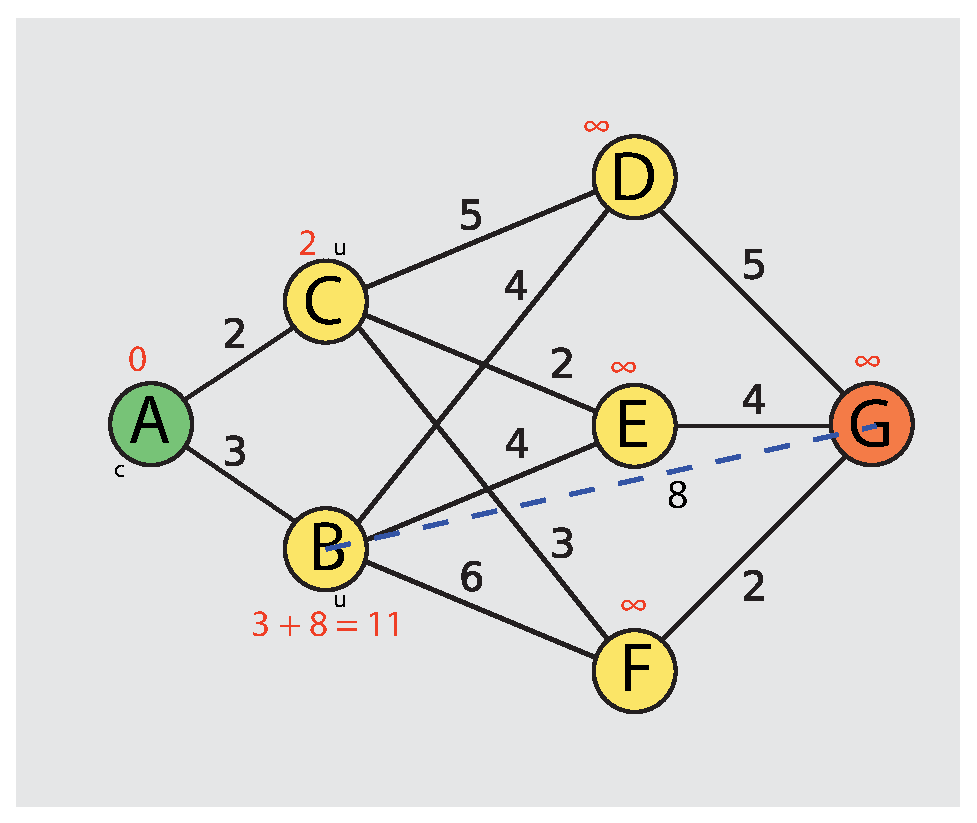
\includegraphics[width=0.5\textwidth]{astar_explained.eps}
    \caption{A*: how is the heuristic value estimated. The dashed line represents the line-of-sight distance.}
    \label{fig:astar_h_explained}
  \end{figure}

  \subsection{Summary of Algorithms}

  There are different kinds of pathfinding problems. These include SSSP and SPSP problems. Dijkstra's algorithm solves SSSP problems and the A* algorithm solves SPSP problems. Dijkstra and A* each have different assets. These are summarized in \cref{tbl:scheme}.
  
  \begin{table}[ht!]
    \centering
  \rowcolors{1}{}{lightgray}
    \begin{tabular}{|r|l|c|}

      \hline
      \textbf{Algorithm} & \textbf{Advantages} & \textbf{Disadvantages} \\
      \hline
      Dijkstra's & Always optimal path & Slow calculation \\
      A* & Optimal path if $h(x)<g(x)$, Fast calculation & Not always optimal path \\
      \hline
    \end{tabular}
    \caption{Table of advantages/disadvantages of different algorithms}
    \label{tbl:scheme}
  \end{table}

  \kanote{indsæt koordinate shizzle}


%!TEX root = ../../Master.tex

\section{Flowchart}

% Define block styles
\tikzstyle{decision} = [diamond, draw, fill=blue!20, text width=4.5em, text badly centered, node distance=3cm, inner sep=0pt]
\tikzstyle{block} = [rectangle, draw, fill=blue!20, text width=5em, text centered, rounded corners, minimum height=4em]
\tikzstyle{line} = [draw, -latex']
\tikzstyle{cloud} = [draw, ellipse, fill=red!20, minimum height=2em]
    
\begin{tikzpicture}[node distance = 4cm, auto]
    % Place nodes
    \node [cloud] (fp) {Find Path};
      \node [decision, below of=fp] (iu) {Is source on same floor as dest.};
        \node [block, right of=iu] (fg) {Perform A* on floor graph};
        \node [block, left of=iu] (exits) {Find exits to destination floor};
          \node [block, below of=exits] (multi) {Perform A* on source and dest. floor to exits};
          \node [block, below of=multi] (costs) {Evaluate total costs};

        \node [cloud, below of=iu] at (4,-7) (return) {Return path};

    % Draw edges
    \path [line] (fp) -- (iu);
    \path [line] (iu) -- node {yes}(fg);
    \path [line] (iu) -- node {no}(exits);
    \path [line] (exits) -- (multi);
    \path [line] (multi) -- (costs);
    \path [line] (fg) -- (return);
    \path [line] (costs) -- (return);

\end{tikzpicture}

The pathfinding solution begins by looking up the floor of source and destination, if both are on the same floor, then perform the A* on the floor graph. Otherwise find all exits on source and destination floor, return cost of shortest exits to exits. When found perform A* from source and destination vertex to exit vertices. Evaluate final shortest path and return.

\sinote{Se robotstøvsuger rapporter om teori. Hvad kan bruges? Strukturmæssigt og forklaringer.}
\sinote{Læs evt. introduction to algorithms}
\sinote{Find ud af hvad en optimal rute er. Er det den korteste distance, eller den korteste travel tid?}

\sinote{Beskriv at vi vil arbejde med lokale relative koordinater}